\subsection{Teilversuch 3: Reflexionsvermögen einer Glasplatte und Brewster Winkel}

	\subsubsection*{Methoden}
		
		\begin{figure}[ht]
			\centering
			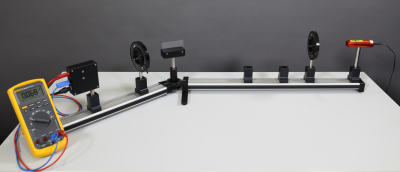
\includegraphics[width=\textwidth]{bilder/Brewster-Winkel.png}
			\caption{Aufbau des dritten Teilversuches\cite{WWU}}
			\label{fig:Glasplatte}	
		\end{figure}
		Der dritte Teilversuch soll wie in Abb. \ref{fig:Glasplatte} dargestellt aufgebaut werden.
		Hier steht statt des $\lambda/2$-Plättchens nun eine Glasplatte in dem Strahlengang.
		Nun soll betrachtet werden wie sich das Reflexionsvermögen der Glasplatte für Einstrahlung von senkrecht bzw. parallel polarisiertem Licht verhält.
		Senkrechtes (s) und paralleles (p) polarisiertes Licht sind die Anteile des polarisierten Lichts, die selbsterklärend senkrecht bzw. parallel zu der Glasplatte eingestrahlt werden.
		Dazu wird die Photodiode an einem Ende und der Laser an dem anderen angebracht, sodass diese an dem beweglichen Gelenk mit der Glasplatte um einen variablen Winkel $\Theta$ versetzt werden können.
		Für die Winkel \SIrange{30}{85}{\degree} soll dafür in \SI{5}{\degree} Schritten die Intensität gemessen werden.
		Besonders ist hierbei der Brewster-Winkel, bei dem der reflektierte und der transmittierte Strahl senkrecht zueinander verlaufen bzw. der E-Feld Vektor ausschließlich senkrecht zu der Einfallsebene schwingt.
		Dadurch spielt in der Messung auch nur der parallele Anteil des Laserlichts eine Rolle.
		Aus dem Snellius'schen Brechungsgesetz folgt für die Brewster-Beziehung dann
		\begin{equation} \label{eq:Brewster}
			\tan{\Theta_\text{B}} = n,
		\end{equation}
		für den Fall dass einer der Brechungsindizes eins entspricht (wie hier bei Luft).
		Die Größe $n$ beschreibt hier dann den Brechungsindex der Glasplatte.

	\subsubsection*{Durchführung}
		
		\begin{figure}[ht]
			\centering
			\includegraphics[width=\textwidth]{data/Spiegel.pdf}
			\caption{Aufgenommene Spannungen in Abhängigkeit des Winkels $\Theta$. Die Spannung ist logarithmisch aufgetragen, um das Minima beim Brewster-Winkel $\Theta_\text{B}$ deutlicher erkennen zu können.}
			\label{fig:GlasplatteWinkel}	
		\end{figure}
		Für die Winkel \SIrange{30+-0,4}{85+-0,4}{\degree} wurden in \SI{5+-0,4}{\degree} die zugehörigen Spannungen an der Photodiode gemessen.
		Diese sind in \ref{fig:GlasplatteWinkel} aufgetragen.
	
	\subsubsection*{Datenanalyse}
		
		Die geringste Spannung unter den Messpunkten ließ sich bei \SI{55+-0,4}{\degree} beobachten.
		Damit liegt der Brewster-Winkel für die Glasplatte bei $\Theta_\text{B} =  \SI{55+-0,4}{\degree}$.
		Einsetzen dieses Winkels in Gl. \ref{eq:Brewster} führt zu dem Brechungsindex $n = \SI{1,5508+-0,0008}{}$ für die Glasplatte.
	
	\subsubsection*{Diskussion}
		
		\begin{figure}[ht]
			\centering
			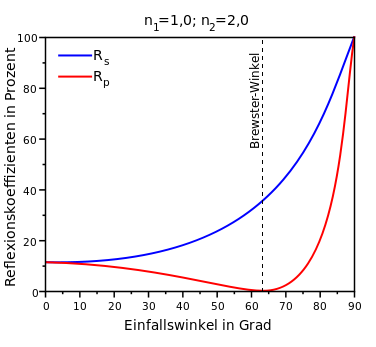
\includegraphics[width=0.6\textwidth]{bilder/wikiBrewster.png}
			\caption{Theoretische Kurve des parallel polarisierten Anteils (rot) bei $n_2 = 2$. \cite{wikiBrewster}}
			\label{fig:wiki_brewster}	
		\end{figure}
		Um zu Überprüfen, ob die gemessenen und ermittelten Werte mit dem bereits Bewiesenem Sachverhalt übereinstimmen, dienen die Abb. \ref{fig:wiki_brewster} und Literaturwerte für den Brechungsindex von Glas.
		Vergleicht man zunächst die aufgenommenen Messpunkte aus Abb. \ref{fig:GlasplatteWinkel} mit der theoretischen Kurve aus Abb. \ref{fig:wiki_brewster}, bei der der Brechungsindex $n_2 = n = 2$ ist, so besitzt der Verlauf des gemessenen Anteils eine ähnliche Form wie die der theoretischen (roten) Kurve.
		Da der aus den Messpunkten ermittelte Brechungsindex bei $n = \SI{1,5508+-0,0008}{}$ liegt, ist eine exakte Übereinstimmung mit der Theorie für $n=2$ jedoch auch nicht zu erwarten gewesen.
		Des Weiteren stellt sich die Frage ob der ermittelte Wert für den Brechungsindex der Glasplatte  einen passenden darstellt.
		Für Kronglas dient der Literaturwert\cite{Refrac} von $n = \SI{1.5145}{}$ und für Flintglas $n = \SI{1.6661}{}$.
		Eine genaue Beschreibung, um welches Glas es sich bei der Platte handelte, war nicht gegeben und zu keinem der beiden Literaturwerte liegt eine genaue Übereinstimmung vor.
		Da der $n$ jedoch zwischen beiden liegt, lässt sich zumindest vermuten, dass die Glasplatte tatsächlich aus einem Glas besteht.
		Ein Widerspruch zu den Fresnel'schen Formeln und der Beugungstheorie lässt sich an dieser Stelle nicht finden.
		
		